\Gls{ibc} systems are a class of data-intensive feedback control systems whose feedback is provided by image-based sensing using a camera. Data-intensive feedback control systems are common nowadays due to advancements in \glspl{cps} \cite{van2018data}. \Gls{ibc} systems have become popular with the advent of efficient image processing algorithms and low-cost \gls{cmos} cameras with high resolution \cite{corke2017robotics}. The combination of the camera and the image processing algorithm gives necessary information on parameters such as relative position, geometry, relative distance, depth perception and tracking of the object-of-interest. Applications of \gls{ibc} are found in robotics \cite{corke2017robotics}, autonomous vehicles \cite{elfring2016effective,pendleton2017perception}, advanced driver assistance systems (ADAS) \cite{bengler2014three}, electron microscopes \cite{FEI}, visual navigation \cite{chakraborty2016compensating} and so on.

As illustrated in Fig.\ \ref{fig:ch5_ibc_bd}, a classical control implementation sequentially and periodically executes the sensing task, control compute task and actuating task. In an \gls{ibc} system, the sensing task has a long, variable execution time, incurring a long delay. Variability in execution time may occur due to variation in image-processing workload and/or in the platform load caused by other applications. The key challenge is to deal with this high dynamic computation demand while guaranteeing performance and meeting safety requirements such as stability. 

\begin{figure}
\vspace*{-1.5ex}
    \centerline{
     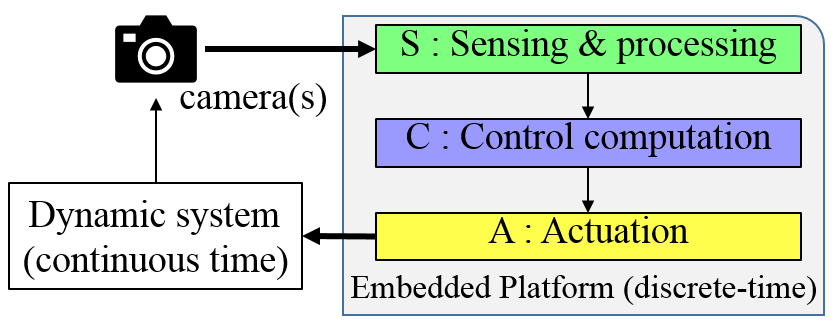
\includegraphics[width=0.6\textwidth]{images/IBC_bd2.png}
    }
    \vspace*{-1.5ex}
    \caption{An \gls{ibc} system: block diagram (repeating Fig.~\ref{fig:ch1_ibc_intro}~(a), for readability)}
    \label{fig:ch5_ibc_bd}
    %\vspace{-2em}
\end{figure}

\Gls{ibc} applications are nowadays usually implemented on some heterogeneous multiprocessor platform that may be shared with other applications.
A typical design flow for \gls{ibc} applications is composed of three distinct elements: (i) \emph{mapping} tasks onto platform resources, which may be done manually or (semi-)automati\-cally; (ii) \emph{timing analysis}, consisting of \emph{task-level} execution-time analysis and \emph{app\-lication-level} analysis to obtain worst-case application-level latency and throughput bounds; (iii) \emph{controller design} ensuring performance and safety guarantees taking into account task- and application-level temporal bounds. A typical flow abstracts variable task execution times through \gls{wcet} estimates. These are often overly conservative, because of image-dependent workload variations and/or difficult to predict platform timing. This leads in turn to loose application-level timing bounds which hampers controller design. The resulting \gls{ibc} system has sub-optimal control performance and is often over-dimensioned.

Fig.\ \ref{fig:ch5_intro} illustrates a standard \gls{ibc} implementation on a single processing core.
A camera captures image frames with a period $\fh$, the inverse of which is referred to as the frame rate. 
The frame rate determines the number of image frames that arrive per time unit, e.g., \gls{fps}.
Typically, the camera frame rate is much higher than the rate at which the frames can be processed on a single core.
Pessimistic task-level \gls{wcet} estimates and  application-level analysis result in over-allocation of processing resources for the worst-case workload and idling for non-worst-case workloads (to keep the sampling period constant). This leads to a long sampling period $h$. 
In the example of Fig.\ \ref{fig:ch5_intro}, with one processing core, we can only process every third image frame, resulting in sub-optimal control performance.

\begin{figure}
\vspace*{-1.5ex}\centerline{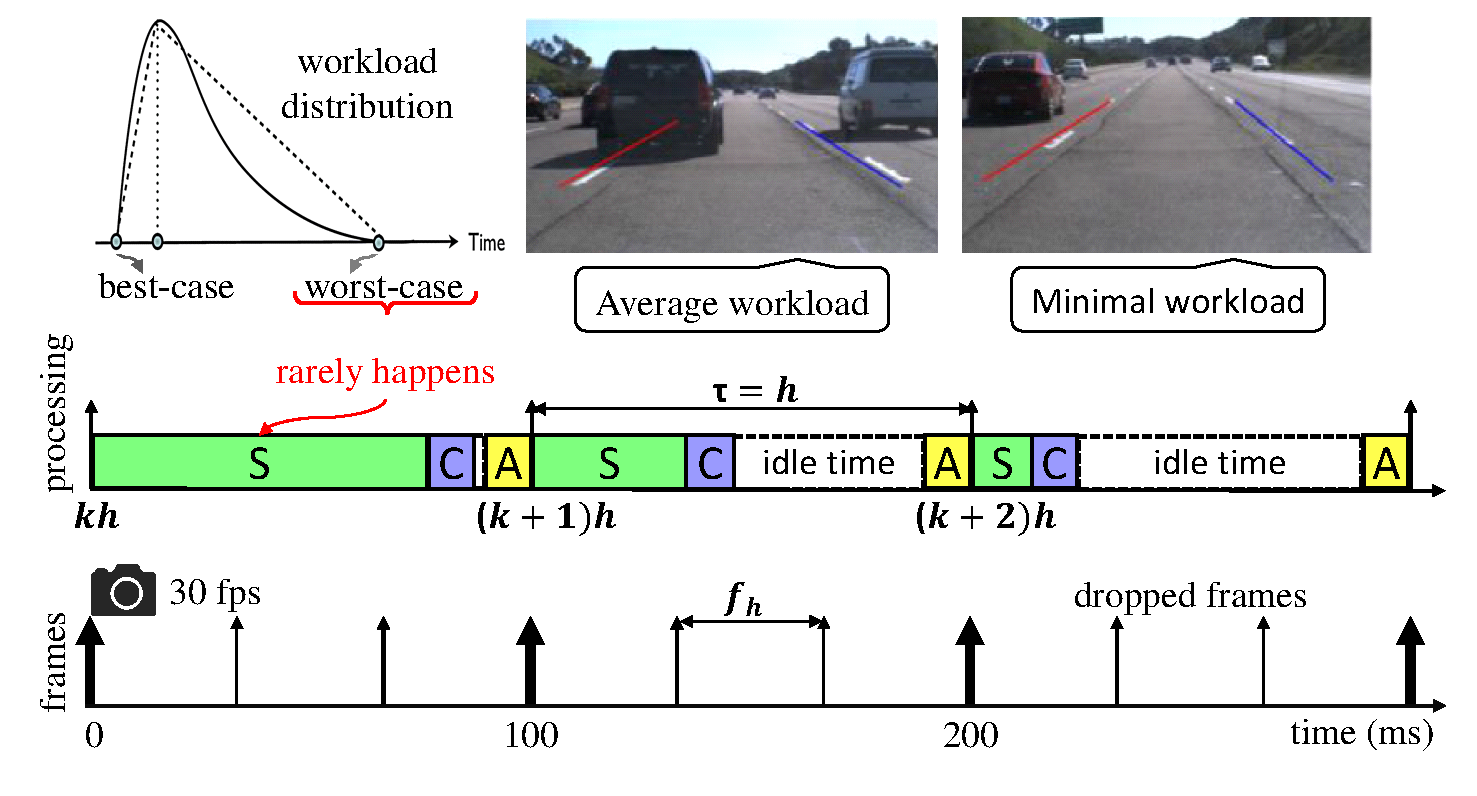
\includegraphics[width=\textwidth]{images/intro.eps}}
\vspace*{-2ex}
\caption{Illustration of classical \gls{ibc} system implementation considering worst-case
scenario. \taskS: sensing and image processing, \taskC: control
computation and \taskA: actuation. (Adapted from Fig. \ref{fig:ch1_ibc_intro} (b) and (c), for readability.)}
\label{fig:ch5_intro}
%\vspace{-2ex}
\end{figure}

\sloppypar
In this chapter, we present the basic version of the model-based \gls{spade} for multiprocessor \gls{ibc} systems, already outlined in Section \ref{chap:spadeoverview}, that exploits \emph{parallelization of the sensing task} and \emph{frequently occurring workload scenarios} to optimize performance. For industrial platforms, where tight task-level \gls{wcet} bounds are difficult to obtain, we moreover propose to use \emph{frequently occurring task execution times} instead of \gls{wcet} estimates to obtain tight, though possibly no longer conservative, application-level temporal bounds for workload scenarios. 
For controller design, we identify appropriate \emph{system scenarios} \cite{gheorghita2009system} that take into account platform mapping and controller performance for specific workload scenarios. Each system scenario corresponds to a specific sampling period. \gls{ibc} performance is then optimized and stability is ensured by designing a \emph{switched controller} that switches at runtime between system scenarios. \Gls{sadf} \cite{theelen2006scenario} is used as a model of computation to capture parallelized (workload and system) scenarios and for timing analysis.

\sloppypar 
Predictable platforms, such as \gls{compsoc} \cite{hansson2009compsoc} and PRET \cite{edwards2007case}, provide predictable tight \glspl{wcet} for individual tasks in an application. Further, the composability property of such platforms ensures that other applications sharing the platform do not interfere with the application under consideration. The \gls{wcet} variations of a task execution on predictable platforms is mainly due to the image workload variations. These properties make predictable \gls{mpsoc} platforms suitable for model-based design. We develop and illustrate our \gls{spade} approach for the predictable and composable interference-free \gls{compsoc} platform. 

We further apply our method on the industrial NVIDIA Drive PX2 platform. Industrial heterogeneous platforms provide high compute power with support for extensive parallelization that is typically needed for data-intensive applications. However, such platforms  are closed-source and use \glspl{os} that result in high variations in execution times of application tasks mapped to the platform.
An ensuing challenge is that the application timing is difficult to predict. Derived task-level \gls{wcet} estimates are overly pessimistic.
Model-based approaches using these pessimistic \glspl{wcet} lead to pessimistic application-level performance bounds. This potentially compromises control performance and may lead to resource over-provisioning. 
However, task execution time distributions due to workload and platform-dependent variations can be statistically analysed from observed data, e.g., as a PERT distribution \cite{adyanthaya2014robustness} (illustrated in Fig.\ \ref{fig:ch5_intro}). Such a distribution allows to classify the most frequently occurring task execution times. Using those  execution times give tighter, though possibly no longer conservative application-level performance bounds. \gls{spade} copes with possible timing analysis violations in the (switched) controller design. Using \gls{spade}, we  perform model-based \gls{dse} for an industrial setup over resource utilisation, quality of control and energy consumption to obtain Pareto-optimal system configurations at design time. We consider the concrete case study of a \gls{lkas} implemented on the NVIDIA Drive PX2 platform, sharing the platform with two other data-intensive applications - object detection and tracking and automatic emergency braking.

\textbf{Contributions:} In this chapter, 
\begin{enumerate}
\item we present the basic \gls{spade} flow for \gls{ibc} system design considering parallel implementation.
    \item we compare \gls{spade} with a state-of-the-art pipelined control approach \cite{medina2019designing} through simulations for a predictable \gls{mpsoc} platform - \gls{compsoc}. Pipelined control does not parallelize the sensing but uses multiple cores to pipeline multiple sensing instances. We provide a guideline when the \gls{spade} approach is suitable with respect to the pipelined control approach. 
    
    \item we adapt \gls{spade} targeting an industrial platform - NVIDIA Drive PX2. We show that we can leverage the principles of predictable model-based \mbox{(co-)}design for industrial platforms by carefully co-designing the image-processing implementation and the switched controller design, using a system-scenario-based approach \cite{gheorghita2009system}.

    \item we validate the \gls{spade} approach in an industrial setting using a \gls{hil} experiment. 
\end{enumerate}